\documentclass{article}
\usepackage{amsmath}
\usepackage{amssymb}
\usepackage{bm}
\usepackage{graphicx}
\usepackage{epstopdf}
\DeclareGraphicsRule{.tif}{png}{.png}{`convert #1 `basename #1 .tif`.png}
\usepackage{color}
\pagestyle{plain}
%\pagestyle{empty}
\textheight 9 true in
\textwidth 6.5 true in
\hoffset -.75 true in
\voffset -.75 true in
 
\mathsurround=2pt  \parskip=2pt
\def\crv{\cr\noalign{\vskip7pt}} 
\def\a{\alpha } \def\b{\beta } \def\d{\delta } \def\D{\Delta } \def\e{\epsilon }
\def\g{\gamma } \def\G{\Gamma} \def\k{\kappa} \def\l{\lambda } \def\L{\Lambda }
\def\th{\theta } \def\Th{\Theta} \def\r{\rho} \def\o{\omega} \def\O{\Omega}
\def\ve{\varepsilon} 

\def\sA{{\cal A}} \def\sB{{\cal B}} \def\sC{{\cal C}} \def\sI{{\cal I}}
\def\sR{{\cal R}} \def\sF{{\cal F}} \def\sG{{\cal G}} \def\sM{{\cal M}}
\def\sT{{\cal T}} \def\sH{{\cal H}} \def\sD{{\cal D}} \def\sW{{\cal W}}
\def\sL{{\cal L}} \def\sP{{\cal P}} \def\s{\sigma } \def\S{\Sigma}
\def\sU{{\cal U}} \def\sV{{\cal V}} \def\sY{{\cal Y}}

\def\gm{\gamma -1}
\def\summ{\sum_{j=1}^4}

\def\bb{{\bm b}} \def\yb{{\bm y}}
\def\ub{{\bm u}}  \def\xb{{\bm x}} \def\vb{{\bm v}} \def\wb{{\bm w}}
\def\omegab{{\bm \omega}} \def\rb{{\bm r}} \def\ib{{\bm i}} \def\jb{{\bm j}}
\def\lb{{\bm l}} \def\kb{{\bm k}} \def\Ab{{\bm A}} \def\fb{{\bm f}} \def\Ub{{\bm U}}
\def\Fb{{\bm F}} \def\nb{{\bm n}} \def\Db{{\bm D}} \def\eb{{\bm e}}
\def\gb{{\bm g}}  \def\Gb{{\bm G}} \def\hb{{\bm h}} \def\Yb{{\bm Y}} \def\Rb{{\bm R}} 
\def\Tb{{\bm T}}

\def\As1{{\bf {\cal A}}_1}\def\DO{{\cal D}_0} \def\UO{{\cal U}_0}
\def\ie{{\it{i.e.}}}

\def\ubbar{{\bf {\bar{u}}}} \def\sbar{{\bar{\sigma }}} \def\ubar{{\bar{u}}}  
\def\abar{{\bar{a}}} \def\vbar{{\bar{v}}}  \def\rbar{{\bar{\rho}}}
\def\pbar{{\bar{p}}} \def\ebar{{\bar{e}}} \def\Tbar{{\bar{T}}}
\def\bbar{{\bar{\beta}}} \def\Mbar{{\bar{M}}}  \def \sMbar{{\bar{\cal M}}}
\def\Ebar{{\bar{E}}} \def\sMbar{{\bar{\cal M}}}
\def\sPbar{{\bar{\cal P}}} \def\xbar{{\bar{x}}}

\newcommand{\pdv}[2]{\frac{\partial#1}{\partial#2}}
\newcommand{\dv}[2]{\frac{d#1}{d#2}}
\newcommand{\ord}[2]{#1^{(#2)}}
\newcommand{\vct}[1]{\vec{#1}}

 \newcommand{\bc}{\begin{center}}
 \newcommand{\ec}{\end{center}}
 
 \newcommand{\bq}{\begin{equation}}
 \newcommand{\eq}{\end{equation}}
 
 \newcommand{\beqs}{\begin{eqnarray}}
 \newcommand{\eeqs}{\end{eqnarray}}
 
 \newcommand{\beqa}{\begin{eqnarray*}}
 \newcommand{\eeqa}{\end{eqnarray*}}
 
 \newcommand{\ol}{\overline}
 \newcommand{\ul}{\underline}
 
 \newcommand{\dint}{{\int \!\! \int \!\!}}
 \newcommand{\tint}{{\int \!\! \int \!\! \int \!\!}}
 
 \newcommand{\bfig}{\begin{figure}}
 \newcommand{\efig}{\end{figure}}
 
 \newcommand{\cen}{\centering}
 \newcommand{\n}{\noindent}
 
 \newcommand{\btab}{\begin{table}}
 \newcommand{\etab}{\end{table}}
 
 \newcommand{\btbl}{\begin{tabular}}
 \newcommand{\etbl}{\end{tabular}}
 
 \newcommand{\bdes}{\begin{description}}
 \newcommand{\edes}{\end{description}}
 
 \newcommand{\benum}{\begin{enumerate}}
 \newcommand{\eenum}{\end{enumerate}}
 
 \newcommand{\bite}{\begin{itemize}}
 \newcommand{\eite}{\end{itemize}}
 
 \newcommand{\cle}{\clearpage}
 \newcommand{\npg}{\newpage}
 
 \newcommand{\bss}{\begin{singlespace}}
 \newcommand{\ess}{\end{singlespace}}
 
 \newcommand{\bhalf}{\begin{onehalfspace}}
 \newcommand{\ehalf}{\end{onehalfspace}}
 
 \newcommand{\bds}{\begin{doublespace}}
 \newcommand{\eds}{\end{doublespace}}
 
 \newcommand{\eps}{\mbox{$\epsilon$}} 
 \newcommand{\stilde}{\mbox{$\tilde s$}} 
 \newcommand{\shat}{\mbox{$\hat s$}} 

 \newcommand{\blue}{\color{blue}}
 \newcommand{\red}{\color{red}}
 \newcommand{\magenta}{\color{magenta}}
 \newcommand{\green}{\color{green}}
 \newcommand{\nc}{\normalcolor}




\pagestyle{empty}
\begin{document}

\begin{center}
\large{ MATH-6620 \hspace{1in}  PERTURBATION METHODS \hspace{1in}SPRING 2016\\ Homework-2 \\ Assigned Tuesday February 9, 2016 \\ Due Friday February 19, 2016}\end{center}
\bigskip

Michael Hennessey

\bigskip

\bc {\bf PROBLEMS} \ec

\benum

\item Consider the function
\begin{equation*}
f(x;\e) = \frac{1+\e x + \sqrt{x+\e}}{1+\sqrt{x+\e e^{-x/\e}}}, \quad x \in [0,1].
\end{equation*}
%
\benum
\item Explain, analytically,  why this function has a layer of thickness
$\e$ at $x=0.$
\item Compute $F_0(x) + \cdots + \e F_1(x) ,$ the outer expansion of $f$ to order $\e.$  This expansion
corresponds to the outer limit process $\e \to 0,$ $x$ fixed.
\item Let $\xi = x/\e.$  Compute $G_0(\xi) + \cdots + \e G_1(\xi),$ the inner expansion of $f$ to order
$\e.$  This expansion corresponds to the inner limit process $\e \to 0,$ $\xi$ fixed.
\item Let $x = \mu \eta$ define an intermediate variable, where $\mu(\e)$ is to be determined.  Find the restrictions on $\mu$ so that $F_0$ and $G_0$ match to order unity (in the intermediate limit), {\it i.e.,}
%
$$\lim_{\e \to 0}[F_0(\mu \eta) - G_0(\mu \eta/\e)] = 0.
$$
%
\item Find the restrictions on $\mu$ so that $F_0 + \cdots + \e F_1$ and $G_0+\cdots + \e G_1$ match to order $\e$ (in the intermediate limit), {\it i.e.,}
%
$$\lim_{\e \to 0}\frac{[\{F_0(\mu \eta) + \cdots + \e F_1(\mu \eta)\}
- \{G_0(\mu \eta/\e) + \cdots + \e G_1(\mu \eta/\e)\}]}{\e} = 0.
$$
%
If the above limit does not exist, then consider relaxing the order of $\e$ to which the two expansions match, and explain the consequences and meaning of such a relaxation.
\eenum

Solution:\\

\benum
\item At $x=0$, we have
$$f(0;\epsilon)=\frac{1+\sqrt{\epsilon}}{1+\sqrt{\epsilon}}=1,$$
possibly stating that there is not a layer at $x=0$, as the function is well-defined there. In this same vein, the function's domain extends beyond $x=0$ in the negative direction. We then take the derivative of $f$ with respect to $x$ to get
$$f'(x;\e)=\frac{-(1-e^{-x/\e})(1+\e x+\sqrt{x +\e})}{2\sqrt{x+\e e^{-x/\e}}(1+\sqrt{x+\e e^{-x/\e}})^2}+\frac{2\e+\frac{1}{\sqrt{x+\e}}}{2+2\sqrt{x+\e e^{-x/\e}}}.$$
If we take the limit as $x$ goes to zero of the derivative, we can finally see why there is a boundary layer at $x=0.$
$$\lim_{x\to 0}f'(x;\e)=\frac{2\e+\frac{1}{\sqrt{\e}}}{2+2\sqrt{\e}}=\frac{2\e^{3/2}+1}{2\sqrt{\e}(1+\sqrt{\e})}\sim O(\e^{-1})>>1.$$
Thus we see there is a layer with thickness $\e$ at $x=0.$

\item We begin by setting $f\sim F_0+...+\e F_1$. We then asymptotically expand $f$ to determine $F_0$ and $F_1$.
    $$F_0=\lim_{\e\to 0}\frac{f}{1}=1.$$
    $$F_1=\lim_{\e\to 0}\frac{f-1}{\e}=\frac{1+\e x+\sqrt{x+\e}-1-\sqrt{x+\e e^{-x/\e}}}{\e(1+\sqrt{x+\e e^{-x/\e}})}\to \frac{x}{1+\sqrt{x}}.$$
    Therefore, our outer expansion is
    $$f\sim1+\e\frac{x}{1+\sqrt{x}}.$$

\item With $\xi=x/\e$, we let $f(x;\e)=G(\xi;\e)\sim G_0(\xi)+...+\e G_1(\xi)$, then we follow the process as in the previous part.
    $$G(\xi;\e)=\frac{1+\e^2\xi+\sqrt{\e(\xi+1)}}{1+\sqrt{\e(\xi+e^{-\xi})}},$$
    $$G_0=\lim_{\e\to 0}\frac{G}{1}=1.$$
    It is easy to see that expanding $G$ directly as $G\sim G_0+\e G_1$ will fail, thus we need an intermediate expansion term. We find this term by expanding $G$ in the same fashion, but we divide by an undetermined power of $\e$.
    $$G_\gamma(\xi)=\lim_{\e\to 0}\frac{G-1}{\e^\gamma}=\frac{\e^2\xi+\sqrt{e}(\sqrt{\xi+1}-\sqrt{\xi+\e^{-\xi}})}{\e^\gamma(1+\sqrt{\e}\sqrt{\xi+e^{-\xi}})}.$$
    We then see that the only way for this limit to be nonzero is if $\gamma=1/2$. Thus we make that choice and get
    $$G_{1/2}=\sqrt{\xi+1}-\sqrt{\xi+e^{-\xi}}.$$
    Fortunately, our choice of $\gamma$ shows us that we are expanding $G$ in half powers of $\e$, therefore we can say our next term in the expansion is $G_1.$
    $$G_1=\lim_{\e\to 0}\frac{G-G_0-\sqrt{\e}G_{1/2}}{\e}=\sqrt{\xi+e^{-\xi}}(\sqrt{\xi+e^{-\xi}}-\sqrt{\xi+1}).$$
    Therefore our inner expansion is
    $$G\sim 1+\sqrt{\e}(\sqrt{\xi+1}-\sqrt{\xi+e^{-\xi}})+\e\sqrt{\xi+e^{-\xi}}(\sqrt{\xi+e^{-\xi}}-\sqrt{\xi+1}).$$

\item If we let $x=\mu\eta$, then $F_0$ and $G_0$ are left unchanged. Therefore in the limit
$$\lim_{\e\to 0}[F_0(\mu\eta)-G_0(\mu\eta/\e)]=1-1=0.$$
Thus there are no restrictions on $\mu$ necessary to match the leading order terms.

\item Now matching to order $\e$ will require a constraint on $\mu.$ We first list $f(\mu\eta)$ and $G(\mu\eta/\e)$:
    $$f(\mu\eta)\sim1+\frac{\e\mu\eta}{1+\sqrt{\mu\eta}};$$
    $$G(\mu\eta/\e)\sim1+\sqrt{\e}(\sqrt{\frac{\mu\eta}{\e}+1}-\sqrt{\frac{\mu\eta}{\e}+e^{-\mu\eta/\e}})+\e\sqrt{\frac{\mu\eta}{\e}+e^{-\mu\eta/\e}}(\sqrt{\frac{\mu\eta}{\e}+e^{-\mu\eta/\e}}-\sqrt{\frac{\mu\eta}{\e}+1});$$
    Then we can show that
    \pagebreak
    $$\frac{F_0+\e F_1-G_0-\sqrt{\e}G_{1/2}-\e G_1}{\e}=\frac{\mu\eta}{1+\sqrt{\mu\eta}}+\frac{\mu\eta}{\e}+e^{-\mu\eta/\e}-\frac{\sqrt{\frac{\mu\eta}{\e}+1}}{\sqrt{\e}}+\frac{\sqrt{\frac{\mu\eta}{\e}+e^{-\mu\eta/\e}}}{\sqrt{\e}}$$
    $$-\sqrt{\frac{\mu\eta}{\e}+1}\sqrt{\frac{\mu\eta}{\e}+e^{-\mu\eta/\e}}.$$
    While it might appear that the limit of this term as $\e\to 0$ is indeterminate or infinite, a bit of trickery shows that the desired result holds for $\mu=o(\e).$ This constraint on $\mu$ results from the ubiquity of the $\mu\eta/\e$ term. Clearly, if we want $\mu\eta/\e$ to go to zero, $\mu=o(\e)$. We now take the limit of the above difference as $\e\to 0$ in a term by term fashion.
    $$\lim_{\e\to 0}\frac{\mu\eta}{1+\sqrt{\mu\eta}}+\frac{\mu\eta}{\e}+e^{-\mu\eta/\e}=0+0+1.$$
    $$\lim_{\e\to 0}-\sqrt{\frac{\mu\eta}{\e}+1}\sqrt{\frac{\mu\eta}{\e}+e^{-\mu\eta/\e}}=-1.$$
    $$\lim_{\e\to 0}\frac{\sqrt{\frac{\mu\eta}{\e}+e^{-\mu\eta/\e}}}{\sqrt{\e}}-\frac{\sqrt{\frac{\mu\eta}{\e}+1}}{\sqrt{\e}}=0.$$
    Then adding these limits together we see that we have a match up to order epsilon, when $\mu=o(\e).$
\eenum
\bigskip
{\bf In each of the following problems, anticipate (if possible) the location of the inner region(s).  You may use the Van Dyke Principle for matching.}

\item For the BVP $\e y'' - y' + \e x^2 y = 2x,\;\; 0<x<1,\;\; y(0;\e)=2,\;\; y(1;\e)=2+\e,$  find the first two terms in the outer and the inner solutions, and the composite approximation.\\

    Solution:\\

    We begin by finding the location of the boundary layer. As the $y'$ coefficient $a(x)=-1$ is negative for all $x$ in our domain, we expect the boundary layer to be located at $x=1.$ We then proceed by finding the first two terms in the outer expansion: $y\sim y_0(x)$, let $\e\to 0.$ Then our differential equation becomes
    $-y_0'=2x.$ The solution to this equation is $y=a_1-x^2.$ This equation should satisfy $y(0;\e)=2$, which implies that $a_1=2.$ Giving us $y_0=2-x^2.$ Then we assume that $y\sim y_0+\e y_1$ and we get a new differential equation
    $$y_0''-y_1'+x^2y_0=0$$ This gives the solution
    $$y_1=-\frac{x^5}{5}+\frac{2}{3}x^3-2x+d_1.$$
    But $y_1(0)=0\implies d_1=0.$ therefore
    $$y_1=-\frac{x^5}{5}+\frac{2}{3}x^3-2x.$$
    Thus we have a two-term outer expansion:
    $$y\sim 2-x^2+\e(-\frac{x^5}{5}+\frac{2}{3}x^3-2x).$$
    Now we find a two-term inner expansion:\\
    We let $1+\delta \xi=x$ and $y(x;\e)=Y(\xi;\e).$ Then our differential equation becomes
    $$\frac{\e}{\delta^2}Y''-\frac{1}{\delta}Y'+\e(1+\delta\xi)^2Y=2(1+\delta\xi)$$
    The dominant balance of the first two terms dictates that $\e=\delta.$ With this, the differential equation becomes
    $$Y''-Y'+\e^2(1+2\e\xi+\e^2\xi^2)Y=2\e+2\e\xi.$$
    Now if we suppose that $Y\sim Y_0$, we only look at the first two terms:
    $$Y_0''-Y_0'=0\implies Y_0=c_1+c_2e^\xi.$$
    Since we should satisfy the right boundary condition with the inner expansion we have
    $$Y(1)=2=c_1+c_2e, \text{ giving }Y_0=2-c_2e+c_2e^\xi.$$
    Then to find the second term of the inner expansion, we take $Y\sim Y_0+\e Y_1$ to get the differential equation
    $$Y_1''-Y_1'=2\implies Y_1=b_1e^\xi+b_2-2\xi, Y_1(1)=1.$$
    Thus the second term of the expansion becomes
    $$Y_1=b_1e^\xi+3-b_1 e-2\xi.$$
    Now we can match the inner and outer expansions:
    $$y_0(x)=2-x^2=y_0(\xi)=2-(1+\e\xi)^2\to 1 \text{ as } \e\to 0,$$
    and
    $$Y_0(\xi)=2-c_2e+c_2e^\xi=Y_0(x)=2-c_2e+c_2e^{(x-1)/\e}\to 2-c_2 e\text{ as }\e\to 0.$$
    Then we see that $1=2-c_2e\implies c_2=1/e,$ and our first term of the inner expansion is $Y_0(\xi)=1+e^{\xi-1}$. Then we match the second term using the same procedure:
    $$y_0+\e y_1=2-x^2+\e(-\frac{x^5}{5}+\frac{2x^3}{3}-2x)\to 1-2\e\xi-\frac{23}{15}\e$$
    and
    $$Y_0+\e Y_1=1+e^{\xi-1}+\e(b_1e^\xi+3-b_1 e-2\xi)\to 3-2x+\e(3-b_1e).$$
    Then $3-2x=1-2\e\xi=1-2(x-1)$ holds and
    $$-\frac{23}{15}=3-b_1 e\implies b_1=\frac{68}{15 e}.$$
    Therefore the inner expansion is
    $$Y_0+\e Y_1=1+e^{\xi-1}+\e(\frac{68}{15}e^{\xi-1}-\frac{23}{15}-2\xi).$$
    Lastly, we form the composite expansion:
    $$y_c=y_0(x)+\e y_1(x)+Y_0(x)+\e Y_1(x)-\text{ 'common part' };$$
    $$y_c=2-x^2+e^{(x-1)/\e}+\e(-\frac{x^5}{5}+\frac{2x^3}{3}-2x+\frac{68}{15}e^{(x-1)/\e}).$$
    For some reason, the $1/e$ coefficient on the inner expansion terms gives an improper result (as verified by plotting the numerical solution and the asymptotic solutions in Mathematica, see attached), therefore it is omitted.


\item  For the BVP $\e y'' + x^{1/3} y' + y^2 = 0,\;-\; 1<x<1,\;y(-1;\e)=2/9,\;\; y(1)=1/3,$  find the leading-order
outer and inner solutions, and the composite approximation.\\

Solution:\\

We first find the boundary layer: $a(x)=x^{1/3}$, changes sign over the interval, but the derivative $a'(x)=x^{-2/3}/3>0$ for all $x$ in the domain implies that we have a layer in the middle. Now we find the leading term of the outer approximation:
We let $y(x)\sim y_0(x)$ and $\e\to 0$, and get the differential equation $x^{1/3}y_0'+y_0^2=0.$
The solution to this equation that satisfies both boundary conditions is
\[y=\left\{\begin{array}{cc}\frac{2}{3x^{2/3}+6}, &-1\leq x<x_0\\ \frac{2}{3x^{2/3}+3},&x_0<x\leq 1\end{array}\right.\]
As we know the boundary layer must lie in the middle at some point and there is a clear discontinuity at $x=0,$ we choose $x_0=0.$ Now we can change variables and determine the leading order inner expansion. Let $x=\delta \xi$, and $y(x;\e)=Y(\xi;\e)$, then we look for a detailed balance in the differential equation
\[\frac{\e}{\delta^2}Y''+\frac{\xi^{1/3}}{\delta^{2/3}}Y'+Y^2=0.\]
The balance must be between the first two terms, and we see that $\delta= \e^ {3/4}.$ Then if $Y\sim Y_0(\xi),$ we solve the differential equation:
\[Y_0''+\xi^{1/3}Y'_0=0,\]
with undetermined boundary conditions that will result from the matching procedure. The solution to the differential equation for $Y_0$ is
\[Y_0=c_1\int_0^\xi e^{-3s^{4/3}/4}ds+c_2.\]
Now we can match the inner and outer leading-order approximations:
\[y_0(x)=\left\{\begin{array}{cc}\frac{2}{3x^{2/3}+6}, &-1\leq x<0\\ \frac{2}{3x^{2/3}+3},&0<x\leq 1\end{array}\right.=y_0(\xi)=\left\{\begin{array}{cc}\frac{2}{3\e^{1/2}\xi^{2/3}+6}, &-1\leq \xi<0\\ \frac{2}{3\e^{1/2}\xi^{2/3}+3},&0<\xi\leq 1\end{array}\right. \to \left\{ \begin{array}{cc}\frac{1}{3}, &-1\leq \xi<0\\ \frac{2}{3}, &0<\xi\leq 1\end{array}\right. \text{ as }\e\to 0\]
\[Y_0(\xi)=c_1\int_0^\xi e^{-3s^{4/3}/4}ds+c_2=Y_0(x)=c_1\int_0^{x\e^{-3/4}}e^{-3s^{4/3}/4}ds+c_2\to \left\{\begin{array}{cc}-c_1\sqrt{\frac{\sqrt{3}}{2}}\Gamma{\frac{3}{4}}+c_2, &-1\leq x<0\\c_1\sqrt{\frac{\sqrt{3}}{2}}\Gamma{\frac{3}{4}}+c_2, &0<x<1\end{array}\right..\]
Then solving the resulting equations for $c_1$ and $c_2$ gives
\[c_1=\frac{1}{6}\sqrt{\frac{2}{\sqrt{3}}}\frac{1}{\Gamma{\frac{3}{4}}},\; c_2=\frac{1}{2}.\]
Then the inner approximation is
\[Y_0=\frac{1}{6}\sqrt{\frac{2}{\sqrt{3}}}\frac{1}{\Gamma{\frac{3}{4}}}\int_0^{x\e^{-3/4}}e^{-3s^{4/3}/4}ds+\frac{1}{2}.\]
We can then form the composite expansion
\[y_c=y_0(x)+Y_0(x)-\left\{\begin{array}{cc}\frac{1}{3}, &-1\leq x<0\\\frac{2}{3}, &0<x\leq 1\end{array}\right.\]
\[y_c=\left\{\begin{array}{cc}\frac{2}{3x^{2/3}+6}+\frac{1}{6}(1+\sqrt{\frac{2}{\sqrt{3}}}\frac{1}{\Gamma{\frac{3}{4}}}\int_0^{x\e^{-3/4}}e^{-3s^{4/3}/4}ds), &-1\leq x<0\\ \frac{2}{3x^{2/3}+3}+\frac{1}{6}(\sqrt{\frac{2}{\sqrt{3}}}\frac{1}{\Gamma{\frac{3}{4}}}\int_0^{x\e^{-3/4}}e^{-3s^{4/3}/4}ds-1), &0<x\leq 1\end{array}\right..\]


\item For the BVP $\e y'' + e^x (xy'-y) = x^2,\;-1<x<1,\;y(-1)=1,\;y(1)=-1,$  find the leading-order
outer and inner solutions, and the composite approximation.  How does the situation alter if the ODE is changed to $\e y'' - e^x (xy'-y) = -x^2$ while the boundary conditions remain the same?\\

Solution:\\

The boundary layer in this problem is not immediately apparent, so we begin by finding the outer solution. We let $y\sim y_0(x)$ and $\e\to 0$ to get the differential equation
$$e^x(xy_0'-y_0)=x^2.$$
This equation has the solution
$$y_0=c_1 x-xe^{-x}.$$
If we attempt to satisfy both boundary conditions we get the outer solution
$$y_0=\left\{\begin{array}{cc}(e-1)x-xe^{-x},&-1<x<x_0\\(e^{-1}-1)x-xe^{-x},&x_0<x<1\end{array}\right.$$
for some $x_0.$ Plotting this function shows there is a discontinuous intersection at $x=0$, showing that we have a corner layer there.
Thus we scale $x=\delta\xi$ and $y(x;\e)=Y(\xi;\e)$ to determine the solution at the inner layer. We determine $\delta$:
$$\frac{\e}{\delta^2}Y''+e^{\delta\xi}(\delta\xi Y'-Y)=\delta^2\xi^2\implies \delta=\sqrt{\e}.$$
The leading order differential equation is then
$$Y_0''-e^{\sqrt{\e}\xi}Y_0=0.$$
The solution is
$$Y_0=a_1 I_0\left(\frac{2\sqrt{e^{\sqrt{\e}\xi}}}{\sqrt{\e}}\right)+a_2K_0\left(\frac{2\sqrt{e^{\sqrt{\e}\xi}}}{\sqrt{\e}}\right).$$
We then attempt to match the inner and outer solutions by introducing the variable $\eta=x/e^\lambda$, and setting $y\sim y_0+\e^\gamma Y_0.$ Then we have
$$y_0(\eta)=\left\{\begin{array}{ccc}(e-1)\e^\lambda \eta-\e^\lambda \eta e^{-\e^\lambda\eta}, &-1<x<0 &\to 0\\(e^{-1}-1)\e^\lambda\eta e^{-\e^\lambda\eta},&0<x<1&\to 0\end{array}\right.$$
$$\e^\gamma Y_0(\eta)=\e^\gamma a_1 I_0\left(\frac{2}{\sqrt{\e}}\sqrt{e^{\e^\lambda \eta}}\right)+\e^\gamma a_2 K_0\left(\frac{2}{\sqrt{\e}}\sqrt{e^{\e^\lambda \eta}}\right)\to 0 \iff a_1=0.$$
However, I cannot determine a constraint on $a_1$ for any values of $\gamma$ or $\lambda.$ The composite solution is then
$$y_c=\left\{\begin{array}{cc}(e-1)x-xe^{-x},&-1<x<x_0\\(e^{-1}-1)x-xe^{-x},&x_0<x<1\end{array}\right.+\e^\gamma a_2 K_0\left(\frac{2}{\sqrt{\e}}\sqrt{e^{x}}\right).$$

If we change the differential equation to $\e y''-e^x(xy'-y)=-x^2,$ the outer solution stays the same, but the location of the boundary layer moves to each endpoint. Thus the outer solution remains as $y_0=c_1x-xe^{-x}$. The inner solution, however must become inner solutions at $x=-1$ and $x=1.$



\item Find the leading-order outer and inner solutions and the composite approximation to the solution of the boundary-value problem
%
$$\e y'' - (1+3x^2)y -x = 0,\;\; 0<x<1,\;\;y(0;\e)=y(1;\e)=1. $$
%
Solution:\\

As $a(x)=0$, we cannot immediately determine where the boundary layer is in this question. Instead, we begin by finding the outer solution. We let $y\sim y_0$ and $\e\to 0$, to get the equation
$$y_0=\frac{-x}{1+3x^2}.$$
However, this equation does not satisfy either boundary condition. Therefore, we can see that there exists a boundary layer at each end of the domain. We begin by finding the inner layer located at $x=0.$ We scale $x=\delta \xi,$ and let $y(x;\e)=Y(\xi;\e),$ and assume $Y\sim Y_0$. Then the differential equation becomes
$$\frac{\e}{\delta^2}Y''-(1+3\delta^2\xi^2)Y-\delta \xi=0.$$
Detailed balance tells us that $\delta=\sqrt{\e}$ and the differential equation for $Y_0$ is
$$Y_0''-Y_0=0, \; Y_0(0)=1.$$
The solution to this equation is
$$Y_0=e^\xi+c_2(e^{-\xi}-e^\xi).$$
We then match on the left:
$$y_0(\xi)=\frac{-\sqrt{\e}\xi}{1+3\e\xi^2}\to 0\text{ as }\e\to 0;$$
$$Y_0(x)=e^{x/\sqrt{\e}}+c_2(e^{-x/\sqrt{\e}}-e^{x/\sqrt{\e}})\to 0\text{ as }\e\to \iff c_2=1.$$
Thus the inner solution is
$$Y_0(x)=e^{-x/\sqrt{\e}}$$
and the composite approximation on the left is
$$y_c=-\frac{x}{1+3x^2}+e^{-x/\sqrt{\e}}.$$

Now we find the inner solution on the right at $x=1.$ We first scale with $x-1=\mu\eta$, and $y(x;\e)=u(\eta;\e)$, to get the differential equation
$$\frac{\e}{\mu^2}u''-(1+3(\mu\eta+1)^2)u-(\mu\eta+1)=0.$$
Balancing all $O(1)$ terms shows that $\mu=\sqrt{\e}$ and the leading order inner differential equation is
$$u_0''-4u_0=1, \; u_0(1)=1.$$
The solution to this differential equation is
$$u_0=(\frac{5}{4}e^{-2}-a_2e^{-4})e^{2\eta}+a_2e^{-2\eta}-\frac{1}{4}.$$
We then match on the right:
$$y_0(\eta)=\frac{-\sqrt{\e}\eta-1}{1+3(\sqrt{\e}\eta-1)^2}\to\frac{-1}{4}\text{ as }\e\to 0;$$
$$u_0(x)=(\frac{5}{4}e^{-2}-a_2e^{-4})e^{2(x-1)/\sqrt{\e}}+a_2e^{-2(x-1)/\sqrt{\e}}-\frac{1}{4}\to \frac{-1}{4}\text{ as }\e\to 0\iff a_2=0.$$
Then $u_0(x)=\frac{5}{4}e^{-2}e^{2(x-1)/\sqrt{\e}}-\frac{1}{4}.$
Then we form the composite solution on the right (ignoring the $e^{-2}$ term as we did in the second question):
$$y_c=\frac{-x}{1+3x^2}+\frac{5}{4}e^{2(x-1)/\sqrt{e}}.$$
Although we may sacrifice exactly satisfying the boundary conditions, it turns out the additive composite of each left and right composite solutions forms a very good approximation of the exact solution. Thus the composite is
$$y_c=\frac{-x}{1+3x^2}+e^{-x/\sqrt{\e}}+\frac{5}{4}e^{2(x-1)/\sqrt{\e}}.$$


\eenum

\begin{figure}
  \centering
  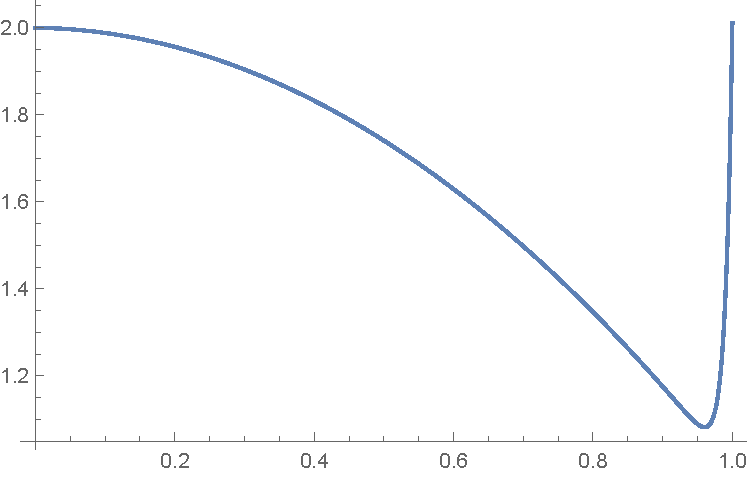
\includegraphics{Perts2numsolve}
  \caption{Numeric solve result from 2}\label{}
\end{figure}

\begin{figure}
\centering
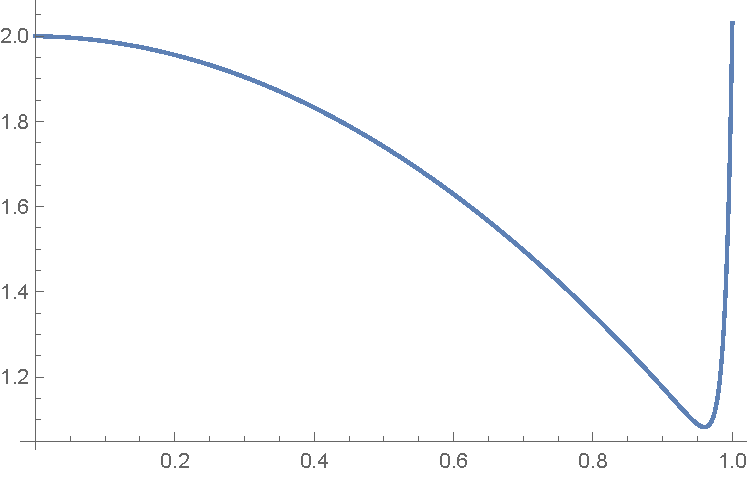
\includegraphics{Perts2asymp}
\caption{Plot of the asymptotic expansion in 2}
\end{figure}

\enddocument} 